\documentclass{beamer}

\usepackage{graphicx}
\usepackage{hyperref}
\usepackage[utf8]{inputenc}
\usepackage[german,english]{babel}
\usepackage[T1]{fontenc}
%\usepackage[english]{babel}
\usepackage{listings}
\usepackage{xcolor,url}
\usepackage{amssymb}
\usepackage{amsmath}
\usepackage{amsfonts}
\usepackage{mathtools}
\usepackage{ifthen}
\usepackage{tcolorbox}
\usepackage{tikz}
\usetikzlibrary{plotmarks}
\usepackage{pgfplots}
\usepackage{upgreek}
\usepackage{dsfont}
\usepackage{framed, color}

\usepackage{metricsbeamer} % using the metric beamer style

\DeclareMathAlphabet{\mathcalbf}{OMS}{cmsy}{b}{n}
%\newcommand{\dd}{\text{d}}
\newcommand{\del}{\partial}

% The command to define a subsection is '\subsec{}' and NOT '\subsection'.
% This code generates the bar. Don't edit.
\newcommand{\midbarnew}{}
\newcommand{\subsec}[1]
{
  \ifthenelse{\equal{#1}{}}
  {\renewcommand{\midbarnew}{} \subsection{}}
  {\renewcommand{\midbarnew}{ $\mid$ } \subsection{#1}}
}

% change the pictures here, if necessary. logobig and logosmall are the internal names
% for the pictures: do not modify them, just change "hulogo" and "logo". Pictures must be 
% supplied as JPEG, PNG or PDF
%########################################

\pgfdeclareimage[height=2cm]{logobig}{hulogo} % use hucase instead for the Humboldt-Case Logo
\pgfdeclareimage[height=1cm]{logosmall}{hulogo}

% use this number to modify the scaling of the headline on titlepage
\def\titlescale{1.3}


\def\authora{Philipp Töpfer}	% First Author
%\def\affa{Humboldt-Universität zu Berlin, Institut für Physik} % First Author's Affiliation
\def\authorb{Dr. Valentina Forini}  % Second Author
%\def\affb{Humboldt-Universität zu Berlin} % Second Author's Affiliation
\def\authorc{Dr. Björn Leder}  % Third Author
%\def\affc{Humboldt-Universität zu Berlin} % Third Author's Affiliation

\def\linka{}	% Link to your institution's/ personal website
\def\linkb{}
\def\linkc{}
\def\email{\href{mailto:your.email@address.com}{your.email@address.com}}	% Your email address

\title[Strings on the lattice and AdS/CFT]{\centering Lattice discretisation of the Green-Schwarz superstring and AdS/CFT \\}
\institute{Humboldt-Universität zu Berlin \\ Emmy Noether Research Group}

% - - - - - - - - - - - - - - - - - - - - - - - - - - - - - - - - - -


%Start of the document
\begin{document}
\Section{}

\frame[plain]{% create the titleslide, layout controlled in metricsbeamer
\vspace{-1.5cm}	\titlepage
}

\Section{Introduction}

\frame{% how to print
\frametitle{Outline}

\begin{tcolorbox}[colback=white!95!black, colframe=white!90!black]
\begin{center}
\textcolor{blue!90}{Lattice} field theory study of \textcolor{blue!90}{AdS/CFT} from a \textcolor{blue!90}{worldsheet string perspective}
\end{center}
\end{tcolorbox}
\hfill \vspace{1mm}



\begin{itemize}
\item<2-> Motivation
\item<2-> AdS/CFT duality
\item<2-> String theory framework
\item<2-> Numerical approach
\item<2-> Results and conclusion
\end{itemize}

}

%###############################################

\Section{Motivation}

%\frame{
%\frametitle{Motivation}
%
%\begin{itemize}
%\item<1-> Good predictions on the real world via QCD
%\item<1-> Fundamental aim: particle masses as functions of parameters\\
%\begin{center} $m_{\rm p} = f(\alpha_{\rm s},\alpha,\mu_{\rm reg},\ldots)$ \end{center}
%\item<2-> Gain more insights on QCD $\leftrightarrow$ study more symmetric model %($\mathcal{N}=4$ SYM)
%\item<2-> $\mathcal{N}=4$ SYM: 
%\begin{itemize}
%\item no massive particles
%\item measure scaling dimensions of local operators and Wilson loops
%\end{itemize}
%\item<3-> Twist two operators:\\
%scaling dimension $\Delta_{S} = 2+S+ \gamma_{S}$\\
%twist \hspace{19mm} $\Delta_{S}-S = 2+ \gamma_{S}$
%\end{itemize}
%}

\begin{frame}
\frametitle{Motivation}
\begin{itemize}
\item Standard Model is most efficient theory of particle physics
\begin{itemize}
\item Unable to incorporate gravity
\item Study $\mathcal{N}=4$ SYM (superconformal version of QCD)
\end{itemize}
\item One of most remarkable discoveries in last decades:\\
{\bf AdS/CFT correspondence} [Maldacena 1997]
\begin{itemize}
\item Relates a superconformal field theory (like $\mathcal{N}=4$ SYM) to a string theory
\item Strong/weak coupling duality
\end{itemize}
\item Study AdS/CFT via the cusp anomaly function ${\color{blue}f(g)}$ from $\mathcal{N}=4$ SYM
\end{itemize}
\end{frame}

%################################################

{\subsec{Cusp anomaly function}

%\begin{frame}
%% mp left
%\begin{minipage}[t]{0.5\linewidth}
%\begin{tcolorbox}[colback=white!95!black, colframe=white!90!black]
%\begin{center}
%\vspace{2.5mm}
%Wilson loop with cusp
%\vspace{2mm}
%\end{center}
%\end{tcolorbox}
%%
%\begin{tcolorbox}[colback=white!95!black, colframe=white!90!black]
%\begin{center}
%$\langle \mathcal{W}[\mathcal{C_{\rm cusp}}]\rangle \sim e^{-\frac{\color{blue}{f(g)}}{2}\vert \phi\vert \ln \frac{L}{\epsilon}}$
%\end{center}
%\end{tcolorbox}
%\end{minipage}
%%
%% mp center
%%
%\begin{minipage}[t]{0.05\linewidth}
%\begin{center}
%\vspace{1.5mm}
%$\Leftrightarrow$
%\end{center}
%\end{minipage}
%%
%% mp right
%%
%\begin{minipage}[t]{0.4\linewidth}
%\begin{tcolorbox}[colback=white!95!black, colframe=white!90!black]
%\begin{center}
%anomalous dimension $\gamma_{S}$
%\end{center}
%\end{tcolorbox}
%%
%\begin{tcolorbox}[colback=white!95!black, colframe=white!90!black]
%\begin{center}
%\vspace{1mm}
%$\gamma_{S} \simeq {\color{blue}f(g)} \ln S$
%\vspace{1mm}
%\end{center}
%\end{tcolorbox}
%\end{minipage}
%%
%%
%%
%\only<1>{
%\begin{center}
%\begin{tikzpicture}[thick,scale=0.5, every node/.style={scale=0.7}]
%\node[anchor=south west,inner sep=0] (image) at (0,0) {\includegraphics[width=0.8\textwidth]{W_cusp.png}};
%\begin{scope}[x={(image.south east)},y={(image.north west)}]
%\node [anchor=west] at (0.69,0.3) {$\mathcal{C_{\rm cusp}}$};
%\node [anchor=south] at (0.072,0.14) {$L$};
%\node [anchor=south] at (0.45,0.78) {$\epsilon$};
%\node [anchor=west] at (0.62,0.82) {$\phi$};
%%\draw[help lines,xstep=.1,ystep=.1] (0,0) grid (1,1);
%%\foreach \x in {0,1,...,9} { \node [anchor=north] at (\x/10,0) {0.\x}; }
%%\foreach \y in {0,1,...,9} { \node [anchor=east] at (0,\y/10) {0.\y}; }
%\end{scope}
%\end{tikzpicture}
%\end{center}
%}
%%
%%
%\only<2>{
%\begin{center}
%via cusp anomaly function
%\end{center}
%\begin{minipage}{0.65\linewidth}
%\begin{tikzpicture}[thick,scale=0.5, every node/.style={scale=0.7}]
%\node[anchor=south west,inner sep=0] (image) at (0,0) {\includegraphics[width=1.1\textwidth]{cusp_anom.png}};
%\begin{scope}[x={(image.south east)},y={(image.north west)}]
%\node [anchor=east] at (0.15,0.92) {$\color{blue} f(g)$};
%\node [anchor=north] at (0.85,0.15) {$\color{blue} g$};
%\node [anchor=south] at (0.75,0.8) {\footnotesize pert. string $\sigma$-model};
%\node [anchor=north] at (0.22,0.17) {\footnotesize pert. gauge theory};
%\node [anchor=east] at (0.5,0.6) {\textcolor{red}{\footnotesize Integrability}};
%\node [anchor=west] at (0.5,0.5) {\textcolor{red}{\footnotesize non-pert. methods}};
%%\draw[help lines,xstep=.1,ystep=.1] (0,0) grid (1,1);
%%\foreach \x in {0,1,...,9} { \node [anchor=north] at (\x/10,0) {0.\x}; }
%%\foreach \y in {0,1,...,9} { \node [anchor=east] at (0,\y/10) {0.\y}; }
%\end{scope}
%\end{tikzpicture}
%\end{minipage}
%%
%%
%\begin{minipage}{0.3\linewidth}
%Here ${\color{blue}g} \equiv \frac{\sqrt{\lambda}}{4\pi} $ \\[3mm]
%t'Hooft coupling\\[2mm]
%$\lambda = g_{\rm YM}^{2}N = \frac{R^{4}}{\alpha'^{2}}$
%
%\end{minipage}
%}
%\end{frame}

\begin{frame}
\vspace{-2mm}
\begin{center}
Cusp anomaly function
\end{center}
\begin{minipage}{0.65\linewidth}
\begin{tikzpicture}[thick,scale=0.5, every node/.style={scale=0.7}]
\node[anchor=south west,inner sep=0] (image) at (0,0) {\includegraphics[width=1.1\textwidth]{cusp_anom.png}};
\begin{scope}[x={(image.south east)},y={(image.north west)}]
\node [anchor=east] at (0.15,0.92) {$\color{blue} f(g)$};
\node [anchor=north] at (0.85,0.15) {$\color{blue} g$};
\node [anchor=south] at (0.75,0.8) {\footnotesize pert. string $\sigma$-model};
\node [anchor=north] at (0.22,0.17) {\footnotesize pert. gauge theory};
\node [anchor=east] at (0.5,0.6) {\textcolor{red}{\footnotesize Integrability}};
\node [anchor=west] at (0.5,0.5) {\textcolor{red}{\footnotesize non-pert. methods}};
%\draw[help lines,xstep=.1,ystep=.1] (0,0) grid (1,1);
%\foreach \x in {0,1,...,9} { \node [anchor=north] at (\x/10,0) {0.\x}; }
%\foreach \y in {0,1,...,9} { \node [anchor=east] at (0,\y/10) {0.\y}; }
\end{scope}
\end{tikzpicture}
\end{minipage}
%
%
\begin{minipage}{0.3\linewidth}
Here ${\color{blue}g} \equiv \frac{\sqrt{\lambda}}{4\pi} $ \\[3mm]
t'Hooft coupling\\[2mm]
$\lambda = g_{\rm YM}^{2}N = \frac{R^{4}}{\alpha'^{2}}$

\end{minipage}
\par
\vspace{2mm}
%Investigate cusp anomaly of $\mathcal{N}=4$ SYM from string theory perspective\\[2mm]
%solve non-trivial 4d QFT with SUSY $\xrightarrow{\color{red} AdS/CFT}{}$ solve non-trivial 2d QFT
\begin{itemize}
\item[] Numerical investigation:\\[2mm]
\begin{minipage}{0.38\linewidth}
\begin{center}
\small solve non-trivial 4d QFT with SUSY
\end{center}
\end{minipage}
\begin{minipage}{0.18\linewidth}
$\xrightarrow{\color{red} AdS/CFT}{}$
\end{minipage}
\begin{minipage}{0.38\linewidth}
\small solve non-trivial 2d QFT
\end{minipage}
\vspace{2mm}
\begin{itemize}
\item More economic memory consumption 
\item Green-Schwarz (GS) approach inherits supersymmetry
\item Only scalar fields involved
\end{itemize}
\end{itemize}
\end{frame}
}

%################################################

\Section{AdS/CFT duality}
\frame{
\frametitle{AdS/CFT duality}

\begin{tcolorbox}[colback=white!95!black, colframe=white!90!black]
\begin{center}
conformal field theory (CFT)
\end{center}
\end{tcolorbox}
%
\begin{equation*}
\uparrow \qquad \textit{dynamically equivalent to} \qquad \downarrow
\end{equation*}\hspace{1mm}
%
%
\begin{tcolorbox}[colback=white!95!black, colframe=white!90!black]
\begin{center}
string theory on background containing Anti-de Sitter (AdS) space as a factor
\end{center}
\end{tcolorbox}

}

%############################################

\frame{
\textbf{Most symmetric setting similar to QCD:} \\[0.3cm]

\begin{tcolorbox}[colback=white!95!black, colframe=white!90!black]
\begin{minipage}{0.70\linewidth}
\begin{center}
\textbf{$\mathcalbf{N}=\mathbf{4}$ SYM}\\
 in 4d, $( g_{\rm YM}, N)$
\end{center}
\end{minipage}
\begin{minipage}{0.20\linewidth}
\includegraphics[scale=0.15]{feynm.png}
\end{minipage}


\end{tcolorbox}
%
\begin{equation*}
\uparrow \qquad \textit{dynamically equivalent to} \qquad \downarrow
\end{equation*}\hspace{1mm}
%
%
\begin{tcolorbox}[colback=white!95!black, colframe=white!90!black]
\begin{minipage}{0.65\linewidth}
\begin{center}
\textbf{Type IIB superstring theory}\\
on $AdS_{5}\times S^{5}$,  $(g_{\rm s},R)$
\end{center}
\end{minipage}
\begin{minipage}{0.15\linewidth}
\includegraphics[scale=0.15]{AdS_S.png}
\end{minipage}
\end{tcolorbox}

}

%##############################################

\frame{
\begin{minipage}{0.25\linewidth}
\begin{tcolorbox}[colback=white!95!black, colframe=white!90!black]
\begin{center}\vspace{3mm}
\textbf{$\mathcalbf{N}=\mathbf{4}$ SYM}
\vspace{3mm}
\end{center}
\end{tcolorbox}
%
%
\begin{tcolorbox}[colback=white!90!red, colframe=white!90!black]
\begin{center}
\vspace{5mm}
$\Uparrow$\\
\textbf{AdS/CFT}\\
$\Downarrow$\\
\vspace{5mm}
\end{center}
\end{tcolorbox}
%
%
\begin{tcolorbox}[colback=white!95!black, colframe=white!90!black]
\begin{center}
\textbf{Type IIB strings}
\end{center}
\end{tcolorbox}
\end{minipage}
%
%
%
\begin{minipage}{0.73\linewidth}
\begin{tcolorbox}[colback=white!95!blue, colframe=white!90!black]
\begin{center}
Wilson loop
\end{center}
$\langle \mathcal{W}[\mathcal{C}]\rangle = \frac{1}{N}{\rm Tr}\,\mathcal{P}\,e^{\oint \left(iA_{\mu}\dot{x}^{\mu}+\phi_{i}\dot{y}^{i}\right) {\rm d}s }$
\end{tcolorbox}
\begin{center}
\begin{tikzpicture}[thick,scale=0.5, every node/.style={scale=0.7}]
\node[anchor=south west,inner sep=0] (image) at (0,0) {\includegraphics[width=0.7\textwidth]{Wilson_loop_worldsheet1.png}};
\begin{scope}[x={(image.south east)},y={(image.north west)}]
\node [anchor=west] at (0.6,0.1) {$\mathcal{C}$};
%\node [anchor=west] at (0.8,0.6) {$\widetilde{\Sigma}$};
%\node [anchor=west] at (0.95,0.1) {$z$};
%\draw[help lines,xstep=.1,ystep=.1] (0,0) grid (1,1);
%\foreach \x in {0,1,...,9} { \node [anchor=north] at (\x/10,0) {0.\x}; }
%\foreach \y in {0,1,...,9} { \node [anchor=east] at (0,\y/10) {0.\y}; }
\end{scope}
\end{tikzpicture}
\end{center}
%
%
%
\begin{tcolorbox}[colback=white!95!blue, colframe=white!90!black]
\vspace{1mm}
${\!\!Z_{\rm string}[\mathcal{C}]\!=\! \int \mathcal{D}X\mathcal{D}h\, e^{-S_{\rm string}(X,h)} \!\sim\! e^{-A_{\rm reg}(\mathcal{C})}}$\\
\vspace{-1mm}
\end{tcolorbox}
\end{minipage}

}

%###############################################

\frame{
\frametitle{Cusp anomaly of $\mathcalbf{N}=\mathbf{4}$ SYM from string theory}
\begin{minipage}{0.6\linewidth}
vev of light-like cusped Wilson loop\\
\begin{tcolorbox}[colback=white!95!black, colframe=white!90!black]
${\!\!\!\langle\mathcal{W}[\mathcal{C}_{\rm cusp}]\rangle \sim e^{-\frac{f(g)}{2}\vert\phi\vert \ln \frac{L}{\epsilon}}, \quad \phi\to\infty}$
\end{tcolorbox}
\end{minipage}
%
\begin{minipage}{0.35\linewidth}
\begin{flushright}
%\begin{tikzpicture}[thick,scale=0.9, every node/.style={scale=0.7}]
%\node[anchor=south west,inner sep=0] (image) at (0,0) {\includegraphics[width=1.2\textwidth]{cusp_worldsheet_vec.png}};
%\begin{scope}[x={(image.south east)},y={(image.north west)}]
%\node [anchor=north] at (0.6,0.37) {$\mathcal{C}_{\rm cusp}$};
%%\draw[help lines,xstep=.1,ystep=.1] (0,0) grid (1,1);
%%\foreach \x in {0,1,...,9} { \node [anchor=north] at (\x/10,0) {0.\x}; }
%%\foreach \y in {0,1,...,9} { \node [anchor=east] at (0,\y/10) {0.\y}; }
%\end{scope}
%\end{tikzpicture}
\vspace{3mm}
\begin{tikzpicture}[thick,scale=0.8, every node/.style={scale=0.7}]
\node[anchor=south west,inner sep=0] (image) at (0,0) {\includegraphics[width=1.5\textwidth]{W_cusp.png}};
\begin{scope}[x={(image.south east)},y={(image.north west)}]
\node [anchor=west] at (0.64,0.3) {$\mathcal{C_{\rm cusp}}$};
\node [anchor=south] at (0.072,0.14) {$L$};
\node [anchor=south] at (0.45,0.78) {$\epsilon$};
\node [anchor=west] at (0.62,0.82) {$\mathit{\Phi}=i\phi$};
%\draw[help lines,xstep=.1,ystep=.1] (0,0) grid (1,1);
%\foreach \x in {0,1,...,9} { \node [anchor=north] at (\x/10,0) {0.\x}; }
%\foreach \y in {0,1,...,9} { \node [anchor=east] at (0,\y/10) {0.\y}; }
\end{scope}
\end{tikzpicture}
\end{flushright}
\end{minipage}
%
\begin{center}
$\Updownarrow$  \textcolor{red}{AdS/CFT}
\end{center}
%
\begin{tcolorbox}[colback=white!95!black, colframe=white!90!black]
$Z_{\rm cusp} = \int \mathcal{D}\delta X \, \mathcal{D}\delta \mathit{\Psi}\; e^{-S_{\rm IIB}(X_{\rm cl}+\delta X, \delta \mathit{\Psi})} = e^{-\frac{f(g)}{2}\frac{V_{2}}{4}}$
\end{tcolorbox}
String partition function with cusp vacuum $\left( V_{2}=\int {\rm d}t{\rm d}s \right)$

}

%##############################################################

\Section{String theory framework}

\frame{
\frametitle{Green-Schwarz string in AdS light-cone gauge}

\begin{itemize}
\item Sigma-model in $AdS_{5}\times S^{5}$ with RR flux\vspace{2mm}
$S = g \int \dd\tau \dd \sigma\,\left[ G \del X \cdot \del X + \bar{\!\mathit{\Theta}} \Gamma (D+F_{5}) \mathit{\Theta}\del X + \ldots \right]$
\vspace{1mm}
\begin{flushright}
\footnotesize [Metsaev Tseytlin 1998]
\end{flushright}
%
\begin{itemize}
\item $X^{\mu}$ - coordinates of 10d target space
\item $\mathit{\Theta}^{1},\, \mathit{\Theta}^{2}$ - anti-commuting Majorana-Weyl spinors
\end{itemize}

\item Fix $\kappa$-symmetry and apply bosonic light-cone gauge \\
$\Rightarrow$ action at most quartic in complex Grassmann fields $\theta^{i}, \eta^{i}$ (remnants of $\mathit{\Theta}$)

\end{itemize}
}

%###############################################################
%
%\begin{frame}
%\frametitle{Linearisation of fermions}
%quartic fermion contributions $\to \mathit{\Psi}^T \mathcal{O}_{\rm F} \mathit{\Psi}$\\
%Apply a Hubbard-Stratonovich transformation\\
%
%\end{frame}
%
%###############################################################

\begin{frame}
\frametitle{Green-Schwarz string in null-cusp background}

\begin{itemize}
\item In Poincaré patch\vspace{2mm}
$\dd s^{2}_{AdS_{5}} = \frac{\dd z^{2} + \dd x^{+}\dd x^{-} + \dd x^{*}\dd x}{z^{2}}, \quad x^{\pm}=x^{3}\pm x^{0}, \quad x=x^{1}+ix^{2}$\vspace{2mm}
classical solution $\big(\tau,\sigma \in (0,\infty)\big)$: surface\vspace{2mm}
\begin{center}
$z = \sqrt{\frac{\tau}{\sigma}},\quad x^{+}=\tau,\quad x^{-}= -\frac{1}{2\sigma}$ 
\end{center}
\vspace{2mm}
bounded by a null cusp \\ ($AdS_{5}$ boundary at $0=z^{2}=-2x^{+}x^{-}$)
%
\item Expand around classical solution + \\{\small $(\tau,\sigma) \to (t,s)=(\ln \tau,\ln \sigma)$}\\
\vspace{2mm}
{\small $S_{\rm cusp} = g\int \dd t\dd s\, \mathcal{L}_{\rm cusp}$}


\end{itemize}
\only<1>{
\vspace{-26mm}
%\begin{flushright}
\hspace{7.4cm}\begin{tikzpicture}[thick,scale=0.9, every node/.style={scale=0.7}]
\node[anchor=south west,inner sep=0] (image) at (0,0) {\includegraphics[width=0.5\textwidth]{cusp_worldsheet_vec.png}};
\begin{scope}[x={(image.south east)},y={(image.north west)}]
\node [anchor=north] at (0.6,0.37) {$\mathcal{C}_{\rm cusp}$};
\node [anchor=east] at (0.43,1.0) {$z$};
\node [anchor=east] at (0.28,0.75) {$x^{+}$};
\node [anchor=west] at (0.95,0.53) {$x^{-}$};
%\draw[help lines,xstep=.1,ystep=.1] (0,0) grid (1,1);
%\foreach \x in {0,1,...,9} { \node [anchor=north] at (\x/10,0) {0.\x}; }
%\foreach \y in {0,1,...,9} { \node [anchor=east] at (0,\y/10) {0.\y}; }
\end{scope}
\end{tikzpicture}
%\end{flushright}
	}
\end{frame} 

%########################################################

\frame{
\frametitle{Green-Schwarz string in null-cusp background}
\only<1>{
Linearising quartic fermion contributions with {\bf Hubbard-Stratonovich transformation}\\[4mm]
\begin{center}
{ $e^{-g \int \dd t \dd s [-\frac{1}{z^{2}}(-6(\eta^{2})^{2}-\cdots )]} \sim \int \mathcal{D}\phi \mathcal{D}\phi^{I} e^{-g\int \dd t \dd s [\frac{12}{z}\eta^{2}\phi +6\phi^{2} +\cdots] }$}
\end{center}
}


{\small \begin{align*}
\mathcal{L}_{\rm cusp} &=  {\left\vert \partial_t {x} + {\tfrac{m}{2}}{x} \right\vert}^2 + \tfrac{1}{{ z}^4}{\left\vert \partial_s {x} -\tfrac{m}{2}{x} \right\vert}^2 + \left(\partial_t {z}^M + \tfrac{m}{2}{z}^M \right)^2 \\ &\quad+ \frac{1}{{ z}^4} \left(\partial_s {z}^M -\tfrac{m}{2}{z}^M\right)^2
+ \phi^2 +\left( \phi_{I}\right)^{2} + \mathit{\Psi}^T \mathcal{O}_{\rm F} \mathit{\Psi} 
\end{align*}}

\only<1>{
\begin{itemize}
\item 8 bosonic coordinates: {\small $x,x^{*},z^{M}\;(M=1,\ldots,6),\; z=\sqrt{z_{M}z^{M}}$}
\item 17 auxiliary fields {\small $\phi, \phi_{I}$ \small $(I=1,\ldots,16)$}
\item 8 fermionic variables {\small $\mathit{\Psi} \equiv (\theta^{i},\theta_{i},\eta^{i},\eta_{i})$, $\theta^{i}=\theta_{i}^{\dagger}$, $\eta^{i}= \eta_{i}^{\dagger}$, $(i=1,\ldots,4)$}
\end{itemize}
	}
	
\only<2>{
{\footnotesize
\vspace{-8mm}
\begin{flalign*}
\!\!\!\!\!\!\!\!\!\!\!\!\!\!\!\!
\mathcal{O}_{\rm F} & =\begin{pmatrix}
0 & i \mathds{1}_{4}\partial_{t} &\!\!\!\!\! -i\rho^{M}\left(\partial_{s}+\frac{m}{2}\right)\frac{{z}^{M}}{{z}^{3}} & 0\\
i \mathds{1}_{4}\partial_{t} & 0 & 0 & \!\!\!\!\!-i\rho_{M}^{\dagger}\left(\partial_{s}+\frac{m}{2}\right)\frac{{z}^{M}}{{z}^{3}}\\
i\frac{{z}^{M}}{{z}^{3}}\rho^{M}\left(\partial_{s}-\frac{m}{2}\right) & 0 & \!\!\!\!\!2\frac{{z}^{M}}{{z}^{4}}\rho^{M}\left(\partial_{s}{x}-m\frac{{x}}{2}\right) & i \mathds{1}_{4}\partial_{t}-A^{T}\\
0 & \!\!\!\!\! i\frac{{z}^{M}}{{z}^{3}}\rho_{M}^{\dagger}\left(\partial_{s}-\frac{m}{2}\right) &i \mathds{1}_{4}\partial_{t}+A & \!\!\!\!\!\!\!\! -2\frac{{z}^{M}}{{z}^{4}}\rho_{M}^{\dagger}\left(\partial_{s}{x}^\ast-m\frac{{x}}{2}^\ast\right)
\end{pmatrix}~,
\raisetag{-8pt}
\end{flalign*}\\\vspace{2mm}
%
\small
$A=-\frac{\sqrt{6}}{z}\phi \mathds{1}_{4} + \frac{1}{z}\tilde{\phi}+\frac{1}{z^{3}}\rho^\ast_{N}\tilde{\phi}^{T}\rho^{L}z^{N}z^{L}+\mathrm{i}\frac{z^{N}}{z^2}\rho^{MN}\partial_{t}z^{M}$
}
	}	
	
}

%#################################################
\Section{Numerical approach}

\begin{frame}
\frametitle{Numerical approach}

Requires calculating expectation values\vspace{2mm}
{
%\begin{align*}
\begin{tcolorbox}[colback=white!95!black, colframe=white!90!black]
\begin{center}
$Z_{\rm cusp} = \int \mathcal{D}\delta X\mathcal{D}\delta \mathit{\Psi} \; e^{-S_{\rm cusp}} = e^{-\frac{f(g)}{2}\frac{V_{2}}{4}}$
\end{center}
\end{tcolorbox} %\\
\begin{center}
$\Downarrow \qquad \qquad \Downarrow$
\end{center}
\begin{tcolorbox}[colback=white!95!black, colframe=white!90!black]
\begin{align*}
\fcolorbox{white!70!black}{white!80!blue}{$\langle S_{\rm cusp} \rangle $} &= \frac{1}{Z_{\rm cusp}} \int \mathcal{D}\delta X\mathcal{D}\delta \mathit{\Psi} \; S_{\rm cusp} e^{-S_{\rm cusp}} \\
&= -g \frac{\dd \ln Z_{\rm cusp}}{\dd g} = \fcolorbox{white!70!black}{white!80!blue}{$g f'(g) \frac{V_{2}}{8}$}
\end{align*}
\end{tcolorbox}
}
\end{frame}

%########################################################

\begin{frame}
\frametitle{Lattice discretisation}
\begin{minipage}{0.65\linewidth}
\begin{tcolorbox}[colback=white!95!black, colframe=white!90!black]
{\small ${\!\!\!\!\!\!\!\langle A \rangle = \tfrac{1}{Z}\int \mathcal{D}\phi\, A[\phi]e^{-S[\phi]}, \quad Z=\int \mathcal{D}\phi\,e^{-S[\phi]}}$}
\end{tcolorbox}% \vspace{2mm}
Discretise the worldsheet with const. lattice spacing $a$ \\
{\small$\mathit{\Lambda}=\lbrace(n_{0},n_{1})\vert n_{\alpha}=0,\ldots,(N_{\alpha}-1)\rbrace$} so that {\small$\xi^{\alpha}=(t,s)\equiv (an_{0},an_{1}) \equiv an$}
\end{minipage}
\begin{minipage}{0.3\linewidth}
\only<1->{
\vspace{-1cm}
\begin{flushright}
\begin{tikzpicture}[scale=1.1]
%flat grid
\draw (-1,-1) rectangle (1,1);
\path (-1,-1) -- node[below]{$t$} (1,-1);
\path (-1,-1) -- node[left]{$s$} (-1,1);
\draw [step=0.5cm,dashed] (-1,-1) grid (1,1);
\node [anchor=north] at (-1,-1.0) {\tiny $a(0,0)$};
\node [anchor=north] at (1,-1.0) {\tiny $a(T-1,0)$};
\node [anchor=south] at (-1,1.0) {\tiny $a(0,L-1)$};
\path (0,0) circle (0.6pt) node[below=2pt, fill=white]{\tiny $(an_{0},an_{1})$};
\foreach \x in {-1,-0.5,...,1}{
	\foreach \y in {-1,-0.5,...,1}{
		\fill (\x,\y) circle (0.6pt);
	}
}
\end{tikzpicture}
\end{flushright}
}
\end{minipage}

%
\begin{itemize}
\item 
\begin{tabbing}
\hspace{3cm}\=\kill
 \textbf{PI measure:} \> discretise fields $\phi \to \phi(n)$ \\ 
   \> $\mathcal{D}\phi \to \prod\limits_{n} \dd \phi(n)$
\end{tabbing} 
\item \textbf{Operators: } $\del_{\alpha}\phi(n) \to \tfrac{1}{a}[\phi(n+\hat{\alpha})-\phi(n)] \Rightarrow S \to S_{\rm discr}$
\end{itemize}\hfill
%\vspace{2mm}
\begin{minipage}{0.6\linewidth}
$\Rightarrow Z_{\rm discr} = \int \prod\limits_{n} \dd\phi(n)\; e^{-S_{\rm discr}[\phi]}\quad\sim$
\end{minipage} 
\begin{minipage}{0.38\linewidth}
multidimensional integral treatable via MC techniques
\end{minipage}
\end{frame}

%#########################################################

\begin{frame}
\frametitle{Monte Carlo simulations in QFT}

\only<1>{
Generate {\color{blue!90}ensemble} of field configurations $\lbrace \phi_{1},\ldots,\phi_{N}\rbrace$ distributed according $P[\phi]=\exp \big(-S_{\rm E}[\phi]\big)/Z$\\[3mm]
{\color{hublue}\bf Ensemble average}
\begin{tcolorbox}[colback=white!95!black, colframe=white!90!black]
\begin{center}
\vspace{-2mm}
{\small $\langle A \rangle = \int \mathcal{D}\phi\, A[\phi] P[\phi] = \frac{1}{N}\sum\limits_{i=1}^{N}A[\phi_{i}] + \mathcal{O}(1/\sqrt{N}) $}
\vspace{-2mm}
\end{center}
\end{tcolorbox}
%
%
%
\begin{itemize}
\item Grassmann fields are integrated out\\
{\small ${\!\!\!\!\!\!\!\!\!\!\!\!\!\!\!\int \mathcal{D}\mathit{\Psi}\, e^{-\mathit{\Psi}^{\rm T}\hat{\mathcal{O}}_{\rm F}\mathit{\Psi}} = {\rm Pf}\big( \hat{\mathcal{O}}_{\rm F} \big) \quad{\color{red} \xrightarrow{!}}\quad \sqrt[4]{\det (\hat{\mathcal{O}}_{\rm F}\hat{\mathcal{O}}_{\rm F}^{\dagger})} \sim \int \mathcal{D}\zeta\mathcal{D}\zeta^{\dagger}\, e^{-\zeta^{\dagger}(\hat{\mathcal{O}}_{\rm F}\hat{\mathcal{O}}_{\rm F}^{\dagger})^{-\frac{1}{4}}\zeta}}$}
\item Pseudofermionic contribution included into $P[\phi]$
\item Include Wilson term to overcome fermion doubling
\item Use rational hybrid Monte Carlo (RHMC) algorithm to generate ensembles
\end{itemize}
}
%
\only<2>{
Generate {\color{blue!90}ensemble} of field configurations $\lbrace \phi_{1},\ldots,\phi_{N}\rbrace$ distributed according $P[\phi]=\exp\big(-S_{\rm E}[\phi] - \zeta^{\dagger}(\hat{\mathcal{O}}_{\rm F}\hat{\mathcal{O}}_{\rm F}^{\dagger})^{-\frac{1}{4}}\zeta\big) /\tilde{Z}$\\[3mm]
{\color{hublue}\bf Ensemble average}
\begin{tcolorbox}[colback=white!95!black, colframe=white!90!black]
\begin{center}
\vspace{-2mm}
{\small ${\langle S_{\rm cusp} \rangle = \int \mathcal{D}\phi\mathcal{D}\zeta\mathcal{D}\zeta^{\dagger}\, S_{\rm cusp}[\phi] P[\phi] = \frac{1}{N}\sum\limits_{i=1}^{N}S_{\rm cusp}[\phi_{i}] + \mathcal{O}(1/\sqrt{N}) }$}
\vspace{-2mm}
\end{center}
\end{tcolorbox}
%
%
%
\begin{center}
\begin{tikzpicture}[thick,scale=0.9, every node/.style={scale=0.5}]
\node[anchor=south west,inner sep=0] (image) at (0,0) {\includegraphics[width=1.3\textwidth]{markov.png}};
\begin{scope}[x={(image.south east)},y={(image.north west)}]
%\node [anchor=north] at (0.6,0.37) {$\mathcal{C}_{\rm cusp}$};
\node [anchor=south] at (0.74,0.89) {$z$};
\node [anchor=south] at (0.46,0.7) {$\phi_{i}$};
\node [anchor=east] at (0.68,0.65) {$x^{+}$};
\node [anchor=west] at (0.95,0.53) {$x^{-}$};
%\draw[help lines,xstep=.1,ystep=.1] (0,0) grid (1,1);
%\foreach \x in {0,1,...,9} { \node [anchor=north] at (\x/10,0) {0.\x}; }
%\foreach \y in {0,1,...,9} { \node [anchor=east] at (0,\y/10) {0.\y}; }
\end{scope}
\end{tikzpicture}
\end{center}
}
\end{frame}

%###############################################

\begin{frame}
\frametitle{Simulation parameters and continuum limit}
\begin{itemize}
\item Parameters in the continuum: $g$, $m$
\item Dimensionless parameters on the lattice:\\
\begin{center}
$g$, $L$ $(T\equiv 2L)$ , $M\equiv ma$
\end{center}
\item Any observable on lattice is function of input parameters\\
\begin{center}
$\langle F_{\rm LAT} \rangle = \langle F_{\rm LAT}(g,L,M) \rangle = \langle F(g) \rangle + \mathcal{O}(L^{-1}) + \mathcal{O}(e^{-LM})$
\end{center}
\item Continuum limit $\langle F(g) \rangle$ obtained via extrapolation to infinite $L$ $(a\to 0)$
\end{itemize}
\end{frame}

%##############################################

\begin{frame}
\begin{itemize}
\item Take cont. limit in controlled way - {\color{blue!90} Line of constant Physics:}
\begin{itemize}
\item Renormalised physical mass in continuum\\
\begin{center}
$m_{x}^{2}(g) = \frac{m^{2}}{2} \big(1- 1/(8g) + \mathcal{O}(g^{-2})\big)\quad {\color{red}(\ast)}$
\end{center}
\item Keep dimensionless physical quantities constant while $a\to 0$\\
\begin{center}
$\frac{V_{2}m_{x}^{2}}{2} \quad \xrightarrow{g \;{\rm fixed}}{} \quad \frac{V_{2}m^{2}}{2} = (LM)^{2} = {\rm const.}$
\end{center}
if ${\small \color{red}(\ast)}$ is also true on the lattice
\end{itemize}\vspace{2mm}
\item Procedure:
\begin{itemize}
\item Fix $g$
\item Fix $LM$ large enough to keep finite volume effects small
\item Evaluate $\langle F_{\rm LAT} \rangle$ for $L=8,10,12,16,\ldots$
\item Extrapolate to $L\to \infty$ to obtain $\langle F(g) \rangle$
\end{itemize}
\end{itemize}

\begin{center}

\begin{tikzpicture}[scale=0.7, every node/.style={scale=0.8}]
\draw (-1,-1) rectangle (1,1);
\path (-1,-1) -- node[below]{\footnotesize $L=5$} (1,-1);
\path (-1.7,-1) -- node[left]{\footnotesize $LM=c,$} (-1.7,1);
\path (-1,1) -- node[above]{\footnotesize $M=c/5$} (1,1);
\draw [step=0.5cm,dashed] (-1,-1) grid (1,1);
%\path (0,0) circle (0.6pt) node[below=2pt, fill=white]{\tiny $(an_{0},an_{1})$};
\foreach \x in {-1,-0.5,...,1}{
	\foreach \y in {-1,-0.5,...,1}{
		\fill (\x,\y) circle (0.6pt);
	}
}
\end{tikzpicture}
\hspace{6mm}
\begin{tikzpicture}[scale=0.7, every node/.style={scale=0.8}]
%flat grid
\draw (-1,-1) rectangle (1,1);
\path (-1,-1) -- node[below]{\footnotesize $L=7$} (1,-1);
\path (-1,1) -- node[above]{\footnotesize $M=c/7$} (1,1);
%\path (-1,-1) -- node[left]{$\sigma$} (-1,1);
\draw [step=0.333cm,dashed] (-1,-1) grid (1,1);
%\path (0,0) circle (0.6pt) node[below=2pt, fill=white]{\tiny $(an_{0},an_{1})$};
\foreach \x in {-1,-0.666,...,1}{
	\foreach \y in {-1,-0.666,...,1}{
		\fill (\x,\y) circle (0.6pt);
	}
}
\end{tikzpicture}
\hspace{6mm}
\begin{tikzpicture}[scale=0.7, every node/.style={scale=0.8}]
%flat grid
\draw (-1,-1) rectangle (1,1);
\path (-1,-1) -- node[below]{\footnotesize $L=9$} (1,-1);
\path (-1,1) -- node[above]{\footnotesize $M=c/9$} (1,1);
%\path (-1,-1) -- node[left]{$\sigma$} (-1,1);
\draw [step=0.25cm,dashed] (-1,-1) grid (1,1);
%\path (0,0) circle (0.6pt) node[below=2pt, fill=white]{\tiny $(an_{0},an_{1})$};
\foreach \x in {-1,-0.75,...,1}{
	\foreach \y in {-1,-0.75,...,1}{
		\fill (\x,\y) circle (0.6pt);
	}
}
\end{tikzpicture}
\end{center}
\end{frame}

%#########################################################
\Section{Results}
{\usefoottemplate{}
\begin{frame}
\frametitle{Mass of the x field}
\begin{minipage}{0.5\linewidth}
\vspace{-20mm}
Fit timeslice correlators 
\begin{align*}
\huge C_{x}(t) &= \frac{1}{L}\sum\limits_{s_{1},s_{2}} \langle x(t,s_{1})x^{*}(0,s_{2})\rangle \\
&\sim {\rm cosh}\big( (\tfrac{T}{2}-t) m_{x{\rm LAT}} \big)
\end{align*}


\hfill\\
\vspace{10mm}
Extract mass via continuum limit\\
$\frac{m_{x \rm LAT}^{2}(L,g)}{M^{2}} = \frac{m_{x}^{2}(g)}{m^{2}} + \mathcal{O}(L^{-1})$
\end{minipage}
\begin{minipage}{0.45\linewidth}
\vspace{-10mm}
\input{plot_coshcorr}\\
\vspace{-6mm}
\input{mx_vs_g_Lm4_2}
\end{minipage}
\end{frame}

%########################################

\begin{frame}
\frametitle{The cusp action}
\begin{itemize}
\item Observe quadratic divergences $\langle S_{\rm cusp}^{(2)}\rangle \sim \frac{V_{2}}{2}(N_{\rm B}-N_{\rm F})$
\item On the lattice study only bosonic part of the action\\
\begin{center}
$\langle S_{\rm LAT} \rangle = g \frac{(LM)^{2}}{4}f'(g) + \frac{c(g)}{2}(2L^{2}), \quad c(g) = N_{\rm B} +\mathcal{O}(g^{-1})$
\end{center}
\end{itemize}
\vspace{4mm}
\only<1>{
\begin{minipage}{0.48\linewidth}
\begin{center}
\vspace{2mm}
\hspace{-5mm}
\input{c_fit.tex}
\end{center}
\end{minipage}
\begin{minipage}{0.48\linewidth}
\begin{center}
\input{Slat-c_g.tex}
\end{center}
\end{minipage}
}
%\only<2>{
%\begin{center}
%\input{Slat-c_g.tex}
%\end{center}
%}
\end{frame}

%#######################################

\begin{frame}
Subtract divergences and match lattice data to continuum plot via $g_{\rm c} = b \cdot g$, $f'(g)=f'(g_{\rm c})_{\rm c}$

\begin{center}
\input{f_prime_Lm4_andLm6.tex}
\end{center}
\end{frame}

%#######################################
}
\Section{Conclusion}

\begin{frame}
\frametitle{Conclusion}

\begin{itemize}
\item<1-> Investigate cusp anomaly of $\mathcal{N}=4$ SYM from string theory perspective\\[2mm]
%solve non-trivial 4d QFT with SUSY $\xrightarrow{\color{red} AdS/CFT}{}$ solve non-trivial 2d QFT
\begin{minipage}{0.38\linewidth}
\begin{center}
solve non-trivial 4d QFT with SUSY
\end{center}
%\begin{tcolorbox}[colback=white!95!black, colframe=white!90!black]
%\begin{center}
%\vspace{-2mm}
%{\small solve non-trivial 4d QFT with SUSY}
%\vspace{-2mm}
%\end{center}
%\end{tcolorbox}
\end{minipage}
\begin{minipage}{0.18\linewidth}
$\xrightarrow{\color{red} AdS/CFT}{}$
\end{minipage}
\begin{minipage}{0.38\linewidth}
solve non-trivial 2d QFT
%\begin{tcolorbox}[colback=white!95!black, colframe=white!90!black]
%\begin{center}
%\vspace{-2mm}
%solve non-trivial 2d QFT
%\vspace{-2mm}
%\end{center}
%\end{tcolorbox}
\end{minipage}
\vspace{2mm}
\begin{itemize}
\item More economic memory consumption 
\item Green-Schwarz (GS) approach inherits supersymmetry
\item Only scalar fields involved
\end{itemize}
\item<2-> Lattice simulation (gauge-fixed GS string, Wilson term, RHMC):
\begin{itemize}
\item Measured observables seem to be in good agreement with expectation at large $g$
\item At small $g$, $\hat{\mathcal{O}}_{\rm F}$ has small eigenvalues $\to$ sign problem,\\
Qualitative agreement to expectation derived from integrability
\end{itemize}
\end{itemize}
\end{frame}

%#############################################
%\usebackgroundtemplate{\centering \includegraphics[height=\paperheight]{BuddhaBrot_light.jpg}}%
\begin{frame}
\begin{center}
{\Huge \color{hublue} \bf Thank you for the attention!}
\end{center}
\end{frame}

\end{document}

